\chapter{Instrukcja do ćwiczenia}


Aplikację należy pobrać z repozytorium dostępnego
\href{https://github.com/jaroslaw-b/ETS2_test_environment}{\underline{pod tym adresem.}}
Do prawidłowego działania aplikacji wymagany jest komputer z zainstalowanymi:
\begin{itemize}
\item Python w wersji 3.6 lub wyższej
\item OpenCV w wersji 3.1.3 lub wyższej Instalacja z użyciem komendy: \textsc{sudo pip3 install opencv-python} %TODO sudo pip3 install opencv-python ok

\item system Linux (najlepiej Ubuntu) z systemem okien X11
\item biblioteka multiprocessing języka Python
\item biblioteka Wnck (zapewnia komunikację aplikacji z systemem okien). Instalacja poleceniem: \textsc{apt-get install python3-gi gir1.2-wnck-3.0}
\item biblioteka uinput służąca do symulacji kontrolera \href{https://github.com/tuomasjjrasanen/python-uinput}{(\underline{link)}} po pobraniu biblioteki instalacja poleceniem: \textsc{sudo pip install python-uinput}.
%TODO python setup.py build  python setup.py install - chyba można też przy użyciu pip3
\item biblioteka mss (multi screenshot). Instalacja przy użyciu komendy \textsc{sudo pip3 install mss}.
\end{itemize}

%TODO instalcja PIP3 sudo pip3 install mss ok
%TODO sudo pip3 install mss ok


Ćwiczenie należy zacząć od instalacji symulatora jazdy Euro Truck Simulator 2. 
Instalacja poprzez platformę \textit{Steam} jest łatwa i~intuicyjna. 
Dane kont są dostępne u prowadzącego. 
Do każdego konta jest przypisana jedna licencja na grę.

Po instalacji należy po raz pierwszy uruchomić grę i ustawić w ustawieniach grafiki wyświetlanie gry w oknie.
Ew. można to zrobić w pliku konfiguracyjnym -- pole \textsc{uset r\_fullscreen}.
Kolejnym krokiem jest odblokowanie konsoli i narzędzi deweloperskich. 
Aby to zrobić należy zmodyfikować plik \textit{config.cfg}, który powinien znajdować się w lokalizacji: \textit{lsriw/.local/share/Euro Truck Simulator 2/}. 
Dwie linijki w pliku:
\begin{itemize}
\item \textsc{uset g\_ developer "0"}
\item \textsc{uset g\_ console "0"}
\end{itemize}

należy zmienić na:

\begin{itemize}
\item \textsc{uset g\_ developer "1"}
\item \textsc{uset g\_ console "1"}
\end{itemize}

Aktywowanie tych opcji pozwoli na swobodny dostęp do konsoli w grze oraz używanie narzędzi deweloperskich udostępnionych przez twórców. 
W~przypadku aplikacji implementowanej w ramach pracy jest to informacja o prędkości pojazdu oraz stanie gry (pauza/gra). %TODO nie do końca jasne, co znaczy "tej". ok

Następnym etapem jest kompilacja programu, który będzie na bieżąco w trakcie gry zapisywał wspomniane dane do pliku.
W~lokalizacji aplikacji znajduje się folder SDK. %TODO powt. folder/folder ok
Tamże należy odnaleźć lokalizację \textit{examples/telemetry} i będąc w nim wykonać polecenie \textsc{make}. %TODO jeszcze po drodze jest examples ok
Plik wykonywalny \textit{telemetry.so} skopiować do lokalizacji gry: \textsc{/home/lsriw/.steam/steam/steamapps/common/Euro Truck Simulator 2/bin/linux\_ x64/plugins}. Jeśli nie ma końcowego folderu - utworzyć.
%TODO nie było folderu plugins - tworzyć ? tak
Ta operacja sprawi, że gra od tej pory przy każdym uruchomieniu będzie tworzyła plik \textit{telemetry.log}, w którym na bieżąco będzie zapisywana prędkość pojazdu i informacja o aktywnej pauzie. Log będzie pojawiał się w folderze \textsc{/home/lsriw/.steam/steam/steamapps/common/Euro Truck Simulator 2/bin/linux\_ x64/}
%TODO gdzie ten log będzie ok

Uruchomić symulator, powinno pojawić się okno z informacją o uruchomieniu narzędzi deweloperskich (\ref{fig:appendix1_dev_tools}).

\begin{figure}
  \centering
  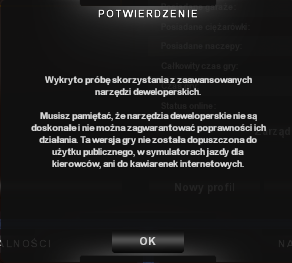
\includegraphics[width=6cm]{img/appendix1_devtools.png}
  \caption{Okno informujące o poprawnym zainstalowaniu SDK}
  \label{fig:appendix1_dev_tools}
\end{figure}

Przy okazji warto przetestować czy konsola również wyświetla się poprawnie. 
Konsolę aktywuje się klawiszem tyldy.

Ważna uwaga! 
Zawsze przed uruchomieniem aplikacji należy uruchomić symulator. 
Przesunięcie okna gry na inny ekran spowoduje niepoprawne działanie aplikacji do testowania algorytmów wizyjnych.

Jeśli wszystkie wymagane biblioteki są zainstalowane, testowo uruchomić aplikację poleceniem \textsc{./run.sh}. 
Aplikacja wymaga dostępu do konta \textit{roota}, ponieważ symulacja kontrolera potrzebuje do niego dostępu. %TODO powt. wymaga ok

Zaleca się korzystanie w grze z kamery numer 6 (klawisz 6).
W bazowej wersji aplikacji, w której nie są zaimplementowane żadne algorytmy wizyjne, obraz przechwycony jest przekazywany do procesu wyświetlającego bez żadnej modyfikacji. %TODO powt. obraz ok
W pliku \textit{Process.py} znajduje się funkcja \textsc{process\_ image(self, image)}. 
Jako argument przyjmuje obraz przechwycony z symulatora. 
Funkcja zwraca listę złożoną z obrazu przetworzonego oraz wektora sterowania: \textsc{return [image, [None, 0, 0]]}. 
W tej funkcji należy implementować algorytmy służące do przetwarzania obrazu. 
Początkowo sugeruje się w ramach testów nie generować sterowania. 
Dopiero po zapewnieniu pewnej stabilności algorytmu zalecane jest najpierw włączenie kontroli kierownicy samochodu, a następnie programowej kontroli prędkości za pomocą symulowanego pedału gazu i hamulca.

Jak wspomniano, początkowo może być trudne generowanie poprawnego (i sensownego) sterowania. 
Aby programowo nie wpływać na kontroler, należy zwracać wektor sterowań w postaci: \textsc{[None, 0, 0]}.

\section{Obsługa kontrolera}

Po zainicjalizowaniu aplikacji gra automatycznie wykryje symulowany kontroler. 
Posiada on trzy osie analogowe służące do sterowania kierownicą oraz pedałami gazu i hamulca. 
Analogowa oś kierownicy posiada zakres $[-32767, 32767]$, gdzie wartości skrajne oznaczają odpowiednio maksymalny skręt w lewo i w prawo. 
W razie nieprawidłowego działania kontrolera należy sprawdzić w ustawieniach, czy okno konfiguracji kontrolera wygląda tak jak na rysunku \ref{fig:appendix1_controller}. %TODO powt. ustawienia ok

\begin{figure}
  \centering
  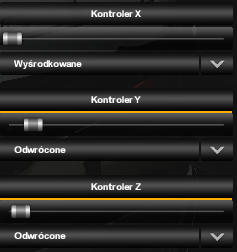
\includegraphics[width=6cm]{img/appendix1_controller.png}
  \caption{Poprawnie zidentyfikowany kontroler}
  \label{fig:appendix1_controller}
\end{figure}

\begin{figure}
  \centering
  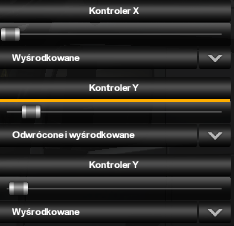
\includegraphics[width=6cm]{img/appendix1_bad_controller.png}
  \caption{Źle zidentyfikowana oś sterowania hamulcem}
  \label{fig:appendix1_bad_controller}
\end{figure}

Czasami, prawdopodobnie w wyniku błędu gry, oś odpowiedzialna za kontrolę hamulca nie jest poprawnie wykrywana (\ref{fig:appendix1_bad_controller}. 
Wtedy należy w ustawieniach kontrolera kliknąć na nazwę osi odpowiedzialną za hamulec i przy uruchomionej aplikacji wpisać:\\ \textsc{import time \\
time.sleep(10)\\
display2control.put([1, None, 100])\\
pass\\}

Zawsze w trakcie pracy aplikacji jest możliwość sterowania ciężarówką za pomocą klawiszy \textbf{W,S,A,D}, co jest przydatne na początku testowania algorytmów wizyjnych.

\section{Obsługa konsoli}
Konsola deweloperska zapewnia możliwość zmiany czasu gry, pogody, prędkości gry oraz lokalizacji. Użyteczne komendy:
\begin{itemize}
\item \textit{g\_ set\_ time hh} -- komenda zmieniająca czas gry, w miejsce \textit{hh} należy wpisać pożądaną godzinę
\item \textit{g\_ set\_ weather x} -- komenda zmieniająca pogodę. W miejsce \textit{x} można wpisać 1 lub 0 (słonecznie lub deszcz)
\item \textit{goto CITY} -- zmienia lokalizację. Później należy jeszcze przeteleportować ciężarówkę klawiszem F9.
\item \textit{warp x} --zmiana prędkości gry. \textit{X} to współczynnik prędkości. Wartości mniejsze od 1 zwalniają symulator, a wartości większe przyspieszają.
\end{itemize}
